\documentclass[11pt,letter,english]{article}
\usepackage{amssymb,babel,colortbl}
\usepackage{hyperref,rotating}
\usepackage{multirow}
\usepackage{color}
\providecommand{\href}[2]{#2}

\oddsidemargin=0mm
\evensidemargin=0mm
\textwidth=160mm
%\textwidth=170mm
%\textheight=232mm
\textheight=9.4in
%\textheight=287mm
\hoffset=0.5cm
%\hoffset=-1.6cm
%\voffset=-0.8cm
\voffset=-2.5cm
%\voffset=-2.4cm
%\documentclass[11pt,letter,english]{article}
%\usepackage{amssymb,babel,colortbl}
%\providecommand{\href}[2]{#2}   
%
%\oddsidemargin=0mm
%\evensidemargin=0mm
%\textwidth=160mm
%\textheight=9.4in
%\hoffset=-0.5cm
%\voffset=-1.2cm

\renewcommand\refname{Bibliography}  

\begin{document}
\nocite{*} 

\small
\newcommand*{\data}{\ifcase\month\or
  January\or February\or March\or April\or May\or June\or
  July\or August\or September\or October\or November\or December\fi
  \space\number\day th,\space\number\year}
%===============================================================================
% New Commands and Definitions
%===============================================================================
\newcommand{\blue}    {\color[named]{Blue}}
\newcommand{\black}   {\color[named]{Black}}
\newcommand{\red}     {\color[named]{Red}}
\newcommand{\green}   {\color[named]{Green}}
\newcommand{\orange}  {\color[named]{Orange}}
\newcommand{\yellow}  {\color[named]{Yellow}}
\newcommand{\magenta} {\color[named]{Magenta}}
\newcommand{\cyan}    {\color[named]{Cyan}}

\def\CP{{\sffamily CP}}

%===============================================================================
% Title
%===============================================================================
\begin{center}
 \section*{\huge{PS-Booster Ejection Correction Dipoles}} 
% \large \textbf{}
 \vspace {0.6cm}
\end{center}

%===============================================================================
% List Of Magnets
%===============================================================================
\subsection*{Goal}

Attempt to reproduce the results in http://wwwpsco.cern.ch/private/gm/gmdescrip/LINC-Note.pdf

\begin{itemize}
\item{Used the latest configuration files for {\bf Ring 3} from Vivien for the ring}
\item{{\bf Matched the optics in MADX (32 bits)} to get the tunes Q$_H=4.17$ and Q$_V=5.23$}
\item{After add a horizontal or vertical kick from one of the correction dipoles}
\item{Compare the closed orbit with the one from the note}
\item{Extract the geometrical relations between the kicks at the entry point and at the center of the ejection Septum, SMH15L1}
\item{Try different configuarions}
\end{itemize}



%===============================================================================
% Head-to-head Comparison
%===============================================================================
\subsection*{Head-to-head Comparison}

\begin{itemize}

\item Configuration 1: {\bf Default 2014 MADX Files}
  \begin{itemize}
  \item DHZ,DVT 4L1 at=1.3355 
  \item DHZ,DVT 11L1 at=0.296 
  \item SMH15L1 4L1 at=0.909892 
  \end{itemize}
\item Configuration 2: {\bf Default 2014 MADX Files, SMH15L1 moved downstream by $\simeq$12 cm}
  \begin{itemize}
  \item DHZ,DVT 4L1 at=1.3355 
  \item DHZ,DVT 11L1 at=0.296 
  \item SMH15L1 4L1 at=0.909892+0.126003
  \end{itemize}

\item Configuration 3: {\bf 2007/2009 Configuration}
  \begin{itemize}
  \item DHZ,DVT 4L1 at=1.426 
  \item DHZ,DVT 11L1 at=0.333 
  \item SMH15L1 4L1 at=0.909892 
  \end{itemize}
\item Configuration 4: {\bf 2007/2009 Configuration, SMH15L1 moved downstream by $\simeq$12 cm}
  \begin{itemize}
  \item DHZ,DVT 4L1 at=1.426 
  \item DHZ,DVT 11L1 at=0.333 
  \item SMH15L1 4L1 at=0.909892+0.126003 
  \end{itemize}

\end{itemize}


\begin{table}[h]

  \caption{
    Comparison for the geometrical relation between the kicks in the different PSB sections at the center of SMH15L1
    }

  \label{tab:geom_rel}
\hspace*{-1.3cm}\begin{tabular}{ |l|c|c|c|c|c| }        \hline
  Kicker & Note Values  & Config. 1 &  Config. 2 & Config. 3 & Config. 4 \\ \hline
         & ``entrance'' & {\bf central}  & {\bf central}  & {\bf central}  & {\bf central}  \\ \hline
  \multirow{2}{*}{BE3.DHZ4L1} & $\Delta$X$_{ES}$[mm]  = 0.760 $\cdot$ DHZ4L1 [mrad] & 0.725 & 0.845 & 0.637 & 0.758\\  \cline{2-6}
                              & $\Delta$X'$_{ES}$[mm] = 0.947 $\cdot$ DHZ4L1 [mrad] & 0.952 & 0.952 & 0.955 & 0.955\\  \hline      
  \multicolumn{6}{|c|}{}        \\ \hline

  \multirow{2}{*}{BE3.DHZ11L1} & $\Delta$X$_{ES}$[mm]  = 5.615 $\cdot$ DHZ11L1 [mrad] & 5.639 & 5.650 & 5.627 & 5.639\\ \cline{2-6} 
                               & $\Delta$X'$_{ES}$[mm] = 0.104 $\cdot$ DHZ11L1 [mrad] & 0.092 & 0.092 & 0.098 & 0.098\\ \hline      
 \multicolumn{6}{|c|}{} \\ \hline

 \multirow{2}{*}{BE3.DVT4L1} & $\Delta$Y$_{ES}$[mm]  = -2.122 $\cdot$ DVT4L1 [mrad] & -2.046 & -2.058 & -2.027 & -2.042\\  \cline{2-6}  
                             & $\Delta$Y'$_{ES}$[mm] =  0.021 $\cdot$ DVT4L1 [mrad] & -0.095 & -0.095 & -0.119 & -0.119\\  \hline       
 \multicolumn{6}{|c|}{} \\ \hline

 \multirow{2}{*}{BE3.DVT11L1} & $\Delta$Y$_{ES}$[mm]  =  0.669 $\cdot$ DVT11L1 [mrad] & 0.350 & 0.248 & 0.374 & 0.273\\     \cline{2-6}  
                              & $\Delta$Y'$_{ES}$[mm] = -0.793 $\cdot$ DVT11L1 [mrad] & -0.806 & -0.806 & -0.803 & -0.803\\ \hline       
 \multicolumn{6}{|c|}{} \\ \hline

\end{tabular}
\end{table}



\begin{table}[h]

  \caption{
    Comparison for the geometrical relation between the kicks in the different PSB sections at the entrance of SMH15L1
    }

  \label{tab:geom_rel}
\hspace*{-1.3cm}\begin{tabular}{ |l|c|c|c|c|c| }        \hline
  Kicker & Note Values  & Config. 1 &  Config. 2 & Config. 3 & Config. 4 \\ \hline
         & ``entrance'' & {\bf entrance}  & {\bf entrance}  & {\bf entrance}  & {\bf entrance}  \\ \hline
  \multirow{2}{*}{BE3.DHZ4L1} & $\Delta$X$_{ES}$[mm]  = 0.760 $\cdot$ DHZ4L1 [mrad] & 0.125 & 0.245 & 0.036 & 0.156\\  \cline{2-6}
                              & $\Delta$X'$_{ES}$[mm] = 0.947 $\cdot$ DHZ4L1 [mrad]  & 0.952 & 0.952 & 0.955 & 0.955\\ \hline      
  \multicolumn{6}{|c|}{}        \\ \hline

  \multirow{2}{*}{BE3.DHZ11L1} & $\Delta$X$_{ES}$[mm]  = 5.615 $\cdot$ DHZ11L1 [mrad] & 5.581 & 5.592 & 5.565 & 5.577\\ \cline{2-6} 
                               & $\Delta$X'$_{ES}$[mm] = 0.104 $\cdot$ DHZ11L1 [mrad] & 0.092 & 0.092 & 0.098 & 0.098\\ \hline      
 \multicolumn{6}{|c|}{} \\ \hline

 \multirow{2}{*}{BE3.DVT4L1} & $\Delta$Y$_{ES}$[mm]  = -2.122 $\cdot$ DVT4L1 [mrad] & -1.986 & -1.998 & -1.952 & -1.967\\  \cline{2-6}  
                             & $\Delta$Y'$_{ES}$[mm] =  0.021 $\cdot$ DVT4L1 [mrad] & -0.095 & -0.095 & -0.119 & -0.119\\  \hline       
 \multicolumn{6}{|c|}{} \\ \hline

 \multirow{2}{*}{BE3.DVT11L1} & $\Delta$Y$_{ES}$[mm]  =  0.669 $\cdot$ DVT11L1 [mrad] & 0.858 & 0.756 & 0.880 & 0.779\\     \cline{2-6}  
                              & $\Delta$Y'$_{ES}$[mm] = -0.793 $\cdot$ DVT11L1 [mrad] & -0.806 & -0.806 & -0.803 & -0.803\\ \hline       
 \multicolumn{6}{|c|}{} \\ \hline

\end{tabular}
\end{table}


%===============================================================================
% To Do
%===============================================================================
\subsection*{ToDo Next}

\begin{itemize}
\item{Introduce the found shift from Tobias Dobers for DVT4L1 and DVT11L1}
\item{Introduce the SMH15L1 values for the blade position from Mike Hourican}
\end{itemize}



%
%\begin{figure}[!hbtp]
%  \begin{center}
%    \includegraphics[width=1.0\textwidth]{figs/LINC-BE_DHZ4L1.png}
%    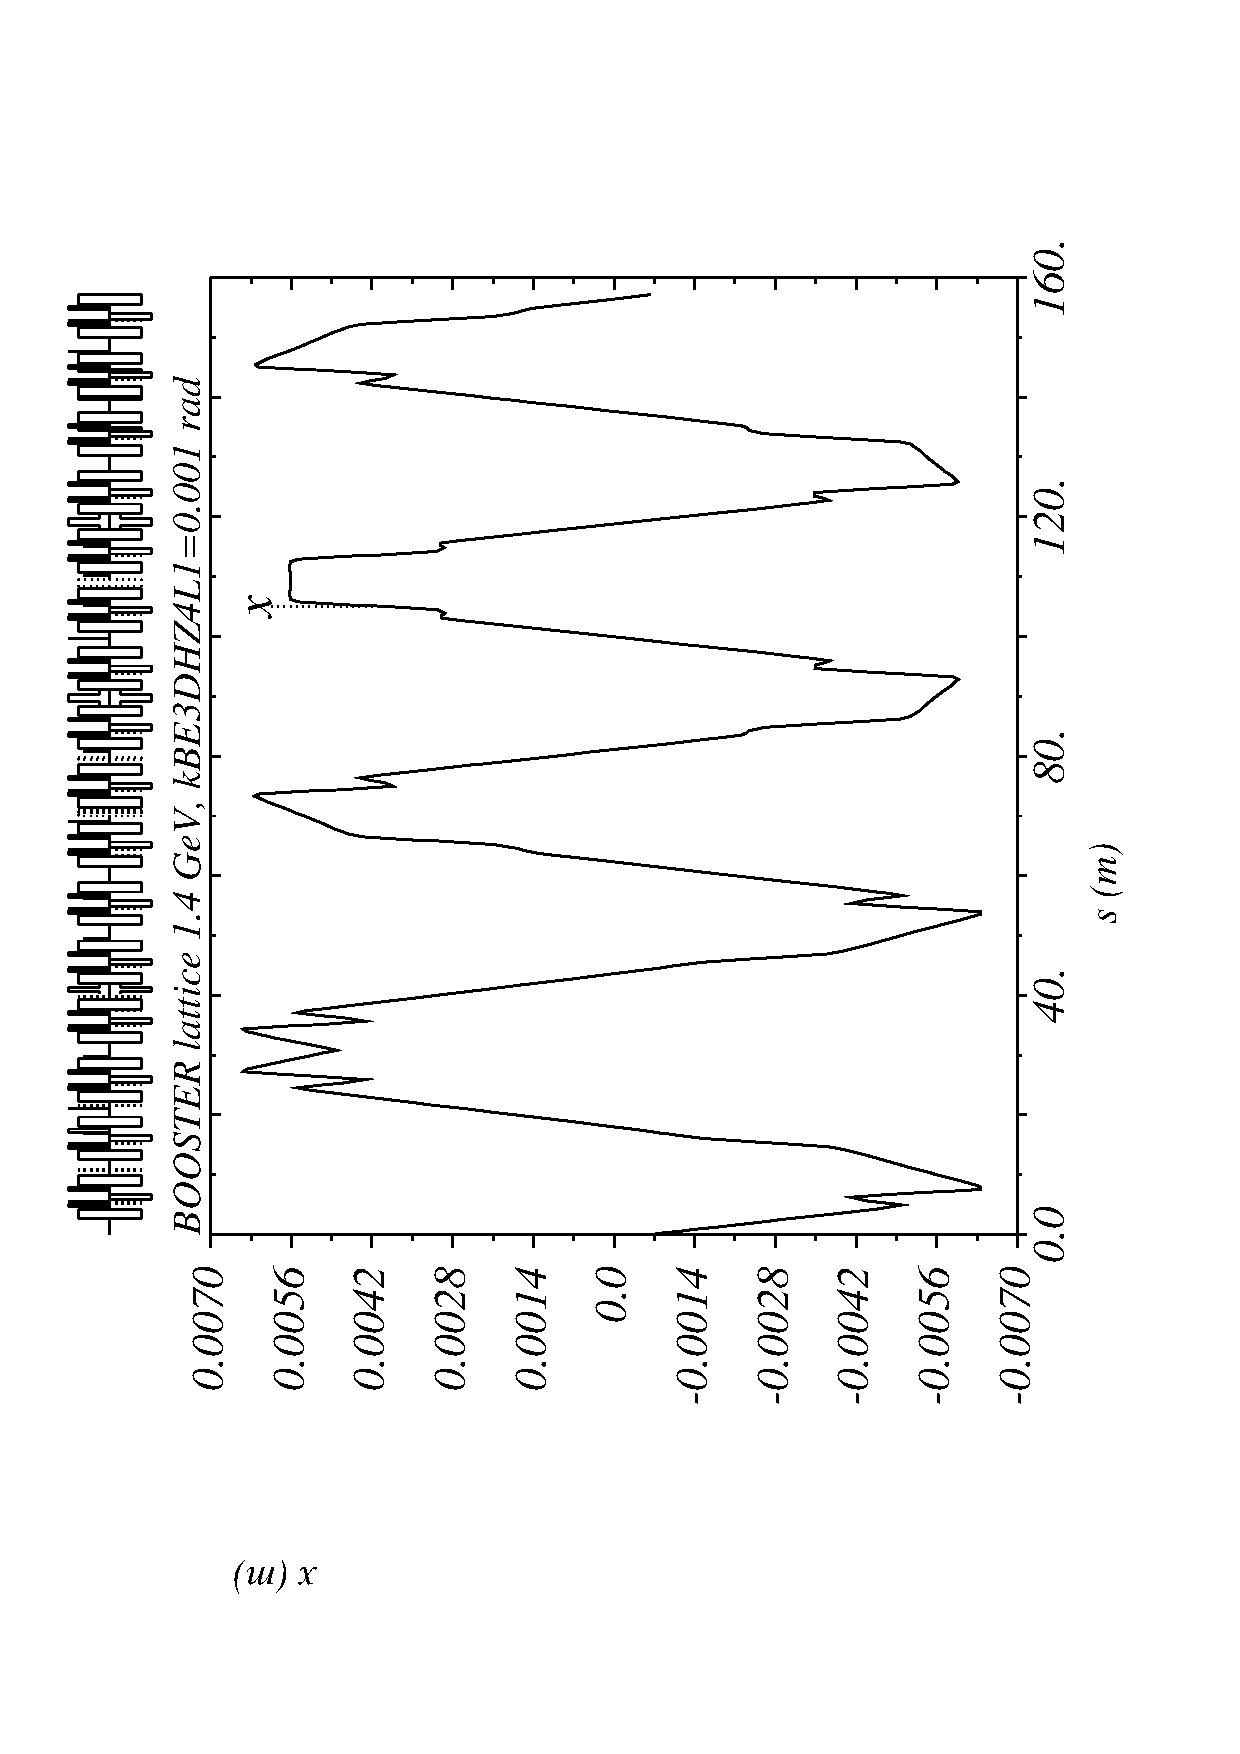
\includegraphics[width=1.0\textwidth]{figs/psb_orbit_BE3DHZ4L1at1mrad.pdf}
%    \caption{Closed Orbit comparison for a kick of 1 mrad for BE3.DHZ4L1. Top: from the note PS/OP/Note 99-xx of M. Benedikt. Bottom: Private MADX files}
%    \label{fig:BE_DHZ4L1}
%  \end{center}
%\end{figure}
%
%
%\begin{figure}[!hbtp]
%  \begin{center}
%    \includegraphics[width=1.0\textwidth]{figs/LINC-BE_DHZ11L1.png}
%    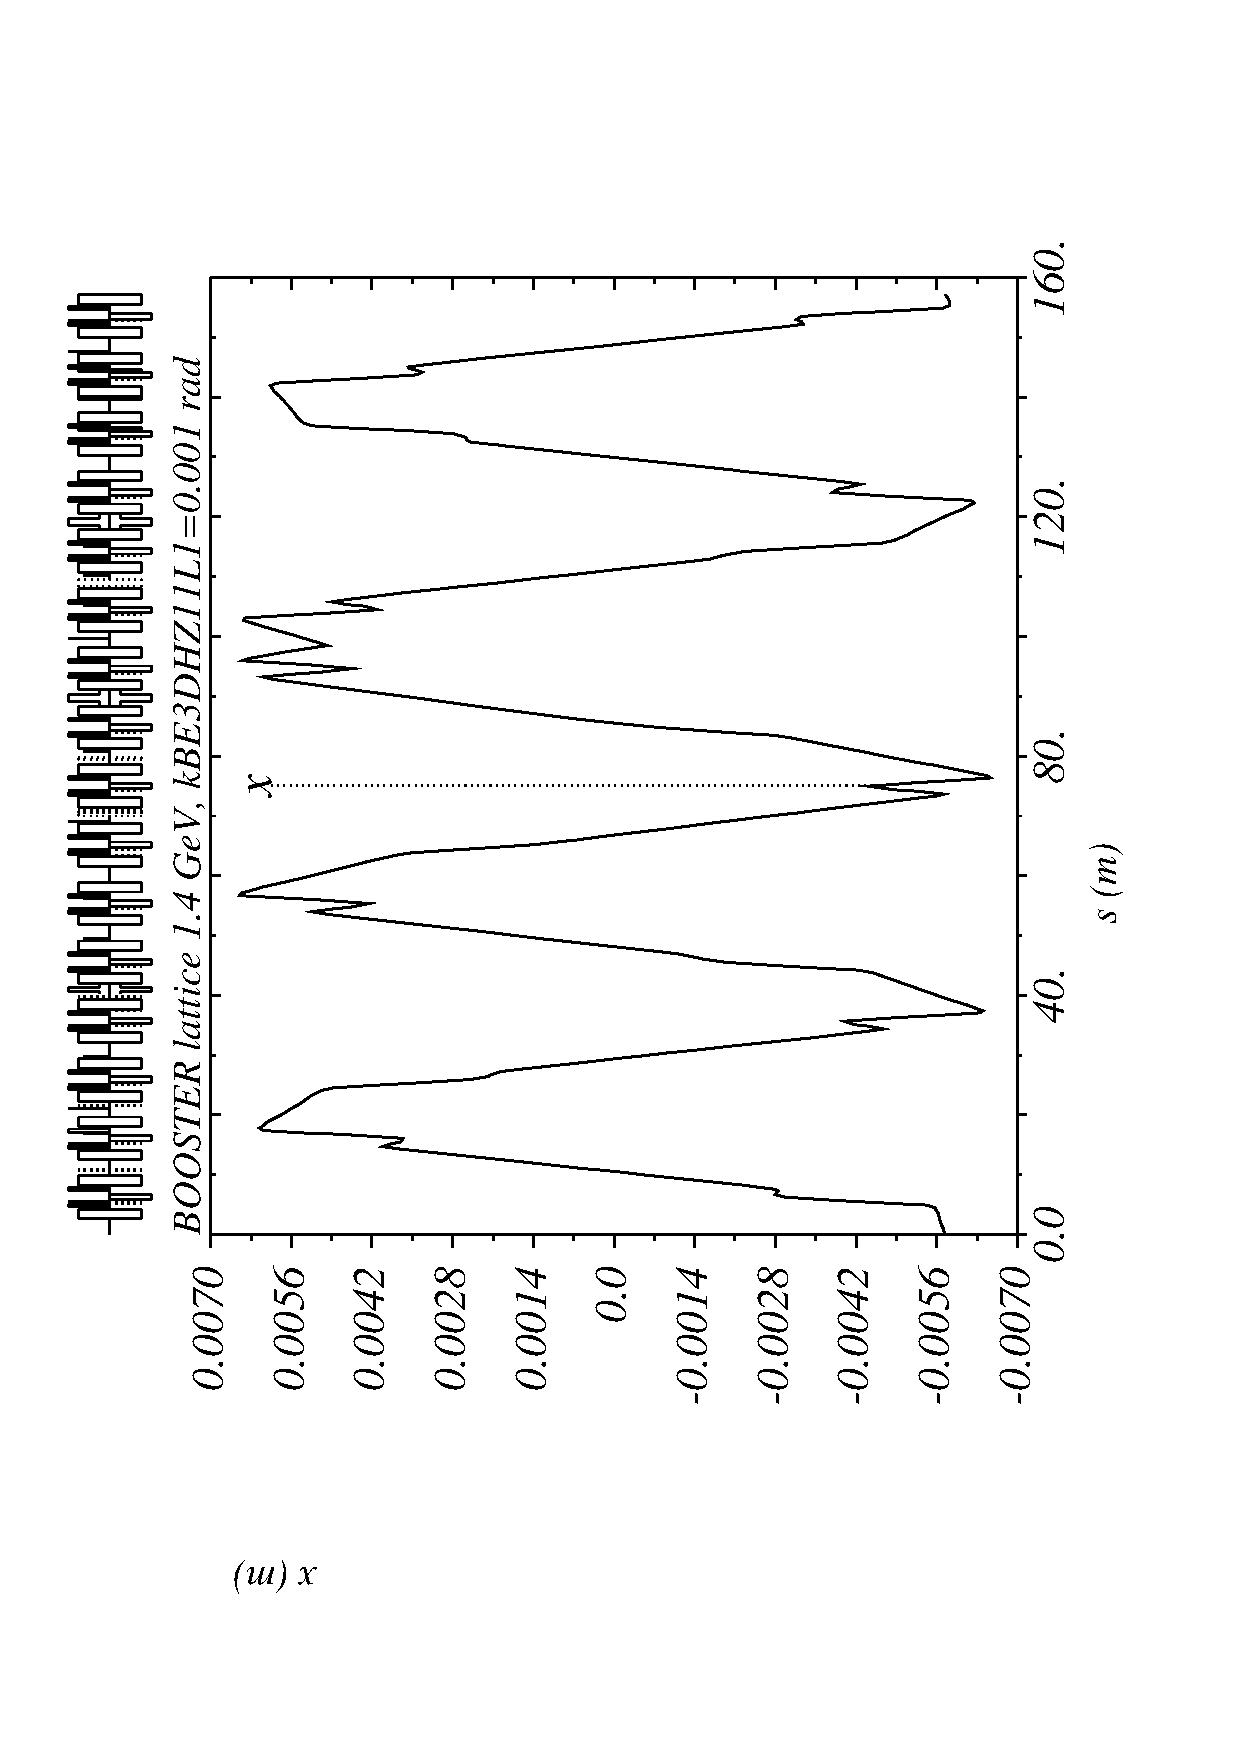
\includegraphics[width=1.0\textwidth]{figs/psb_orbit_BE3DHZ11L1at1mrad.pdf}
%    \caption{Closed Orbit comparison for a kick of 1 mrad for BE3.DHZ11L1. Top: from the note PS/OP/Note 99-xx of M. Benedikt. Bottom: Private MADX files}
%    \label{fig:BE_DHZ11L1}
%  \end{center}
%\end{figure}
%
%
%\begin{figure}[!hbtp]
%  \begin{center}
%    \includegraphics[width=1.0\textwidth]{figs/LINC-BE_DVT4L1.png}
%    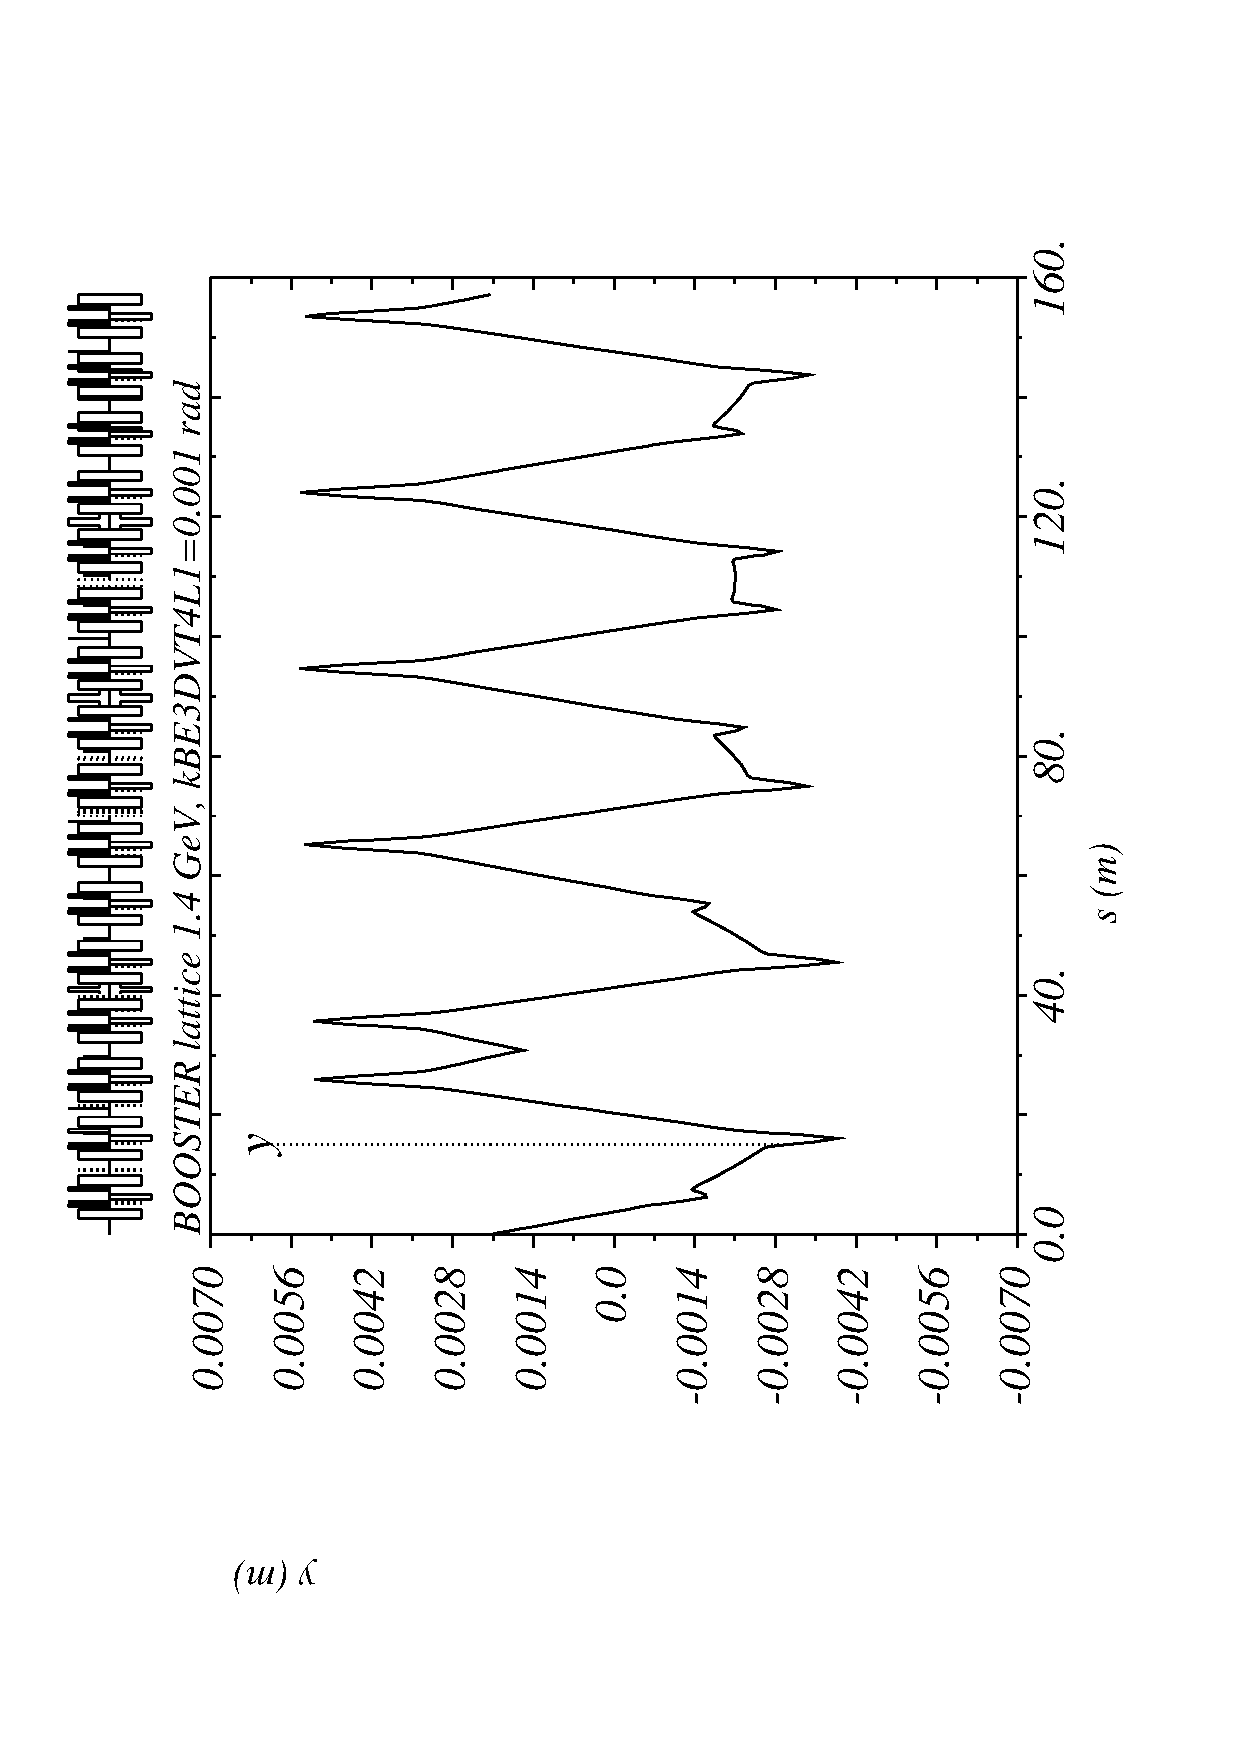
\includegraphics[width=1.0\textwidth]{figs/psb_orbit_BE3DVT4L1at1mrad.pdf}
%    \caption{Closed Orbit comparison for a kick of 1 mrad for BE3.DVT4L1. Top: from the note PS/OP/Note 99-xx of M. Benedikt. Bottom: Private MADX files}
%    \label{fig:BE_DVT4L1}
%  \end{center}
%\end{figure}
%
%
%\begin{figure}[!hbtp]
%  \begin{center}
%    \includegraphics[width=1.0\textwidth]{figs/LINC-BE_DVT11L1.png}
%    \includegraphics[width=1.0\textwidth]{figs/psb_orbit_BE3DVT11L1at1mrad.pdf}
%    \caption{Closed Orbit comparison for a kick of 1 mrad for BE3.DVT11L1. Top: from the note PS/OP/Note 99-xx of M. Benedikt. Bottom: Private MADX files}
%    \label{fig:BE_DVT11L1}
%  \end{center}
%\end{figure}
%
%
%
%%===============================================================================
%% To Do
%%===============================================================================
%\subsection*{Questions}
%
%\begin{itemize}
%\item{Do the results change for the 4 rings? {\bf No, is it expected?}}
%\item{Does the position of the kicker matter? {\bf Yes. E.g., by moving DHZ4L1 4 cm towards the beam I get much closer values of the ones in the note.}}
%\item{Which is the desired level of agreement? {\bf To be discussed with Bettina/Vivien. It is difficult for me to judge without errors associated to estimations}}
%\item{Where to estimate the geometrical relations? {\bf the note says ``entrance of the ejection septum'', although I think they used the center. I tried at the beginning of SMH15L1, but got not compatible values}}
%\end{itemize}





\end{document}


